\documentclass[tikz,border=10pt]{standalone}
\usetikzlibrary{arrows.meta}
\pagecolor{white}
\begin{document}
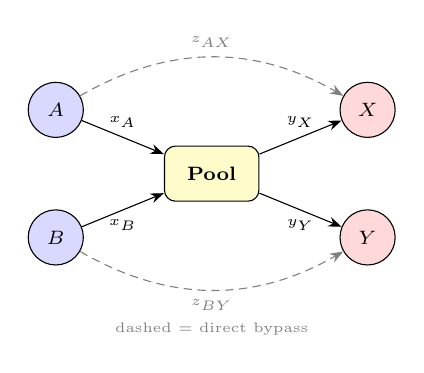
\begin{tikzpicture}[scale=0.9,
  src/.style={circle,draw,fill=blue!15,minimum size=0.7cm,font=\scriptsize\bfseries},
  pool/.style={rectangle,draw,rounded corners=4pt,fill=yellow!20,
               minimum width=1.2cm,minimum height=0.7cm,font=\scriptsize\bfseries},
  prod/.style={circle,draw,fill=red!15,minimum size=0.7cm,font=\scriptsize\bfseries},
  arr/.style={-{Stealth},thin},
]
  \node[src]  (s1) at (0, 2.2) {$A$};
  \node[src]  (s2) at (0, 0.4) {$B$};
  \node[pool] (pl) at (2.2, 1.3) {Pool};
  \node[prod] (p1) at (4.4, 2.2) {$X$};
  \node[prod] (p2) at (4.4, 0.4) {$Y$};
  \draw[arr] (s1) -- node[above,font=\tiny]{$x_A$} (pl);
  \draw[arr] (s2) -- node[below,font=\tiny]{$x_B$} (pl);
  \draw[arr] (pl) -- node[above,font=\tiny]{$y_X$} (p1);
  \draw[arr] (pl) -- node[below,font=\tiny]{$y_Y$} (p2);
  \draw[arr,densely dashed,gray] (s1) to[bend left=30]
    node[above,font=\tiny,pos=0.5]{$z_{AX}$} (p1);
  \draw[arr,densely dashed,gray] (s2) to[bend right=30]
    node[below,font=\tiny,pos=0.5]{$z_{BY}$} (p2);
  \node[font=\tiny,gray] at (2.2,-0.9) {dashed = direct bypass};
\end{tikzpicture}
\end{document}
